\chapter{Introduction}
Drones has a wide variety of potential uses, such as search and rescue, inspection, security, surveillance, research, aerial photography, unmanned cargo systems, military applications, the list goes on. Drones are already widely used, and while some of the aforementioned applications raises ethical issues for debate, there is no doubt that drones also hold a place in the future.

Multicopters constitutes a class of drones with fixed-pitch propellers. This means that the actuation is achieved from a difference in speed between the propellers. Among the all the different varieties of multicopters, see some examples on \autoref{fig:multicopters}, the quadcopter is the most popular, largely due to a compromise between stabilization capabilities and cost of hardware. \cite{TypesOfMulticopter}

\begin{figure}[H]
  \centering
  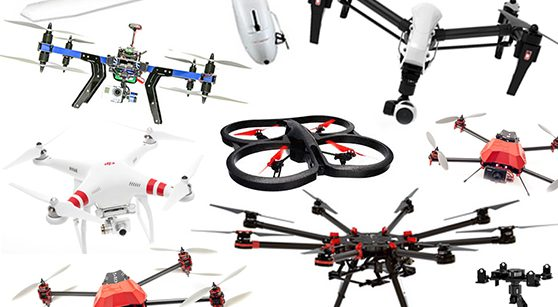
\includegraphics[width=.6\linewidth]{figures/multicopters}
  \caption{A small selection of drones which belongs to the large class of multicopters. \cite{multiCopterPhoto}}
  \label{fig:multicopters}
\end{figure}

The aim of the project is to investigate the capabilities of a specific design strategy when controlling the attitude of a quadcopter as part of a distributed system.

The quadcopter obtains its attitude over a network from a motion tracking system. This introduces delay and packet loss as a limiting factor to the control system situated on the quadcopter. The controlling code is implemented in C on a microcontroller using a real time operating system (RTOS), called FreeRTOS.

The system's coupled behavior and instability raises a challenging control task. This task is solved by implementing a controller design, which is based upon a model that is derived by first principle modeling. This is later linearized since it is desired to use linear controllers.\\
The system is divided into an attitude controller and translational controllers. The attitude controller is in focus in this project. The translational controllers are cascaded around the attitude controller.

The attitude control strategy is based in state space design, and makes use of state feedback, a linear quadratic regulator (LQR) and an integral controller.\\
The translational controllers are designed as classical proportional and integral controllers around the inner state space design.